\documentclass[12pt]{article}
\usepackage{fontspec}
\usepackage{xeCJK}
\setCJKmainfont[AutoFakeBold=2]{SimSun}
%\setCJKsansfont{SimHei}
\usepackage{amsmath, amssymb, amsthm}
\usepackage{geometry}
\usepackage{tikz}
\usepackage{fancyhdr}
%\setlength{\headheight}{15pt}
\usetikzlibrary{calc, intersections} % ABX 用於某些符號，若無可刪除
\usepackage{enumitem}
\usepackage{tkz-euclide}
\usepackage[most]{tcolorbox}
\usepackage{float}
\usepackage{tabularx}
\usepackage{graphicx}
% 定段落首行縮進（兩個中文字）
\setlength{\parindent}{2em}
%\setlength{\parskip}{1em}
\setlength{\headheight}{15pt} % 避免頁首高度警告
\newtcolorbox{mybox}[4][證明]{
  empty,
  breakable,                % 支援跨頁
  sharp corners,
  left=#2+#3,               % 為左側標籤預留空間 (縮進)
  right=0pt, top=0pt, bottom=0pt,
  colback=white,
  % --- 加入以下這行來調整段距 ---
  before upper={\setlength{\parskip}{1em plus 0.2em minus 0.1em}},
  after={\vspace{#4}},
  % ---------------------------
  overlay unbroken and first={ % 在第一頁/未斷頁時繪製標籤
    \node[
      anchor=north west,
      draw, 
      inner sep=0pt,
      minimum width=#2,
      minimum height=1.6em, 
      font=\bfseries\boldmath
    ] at (frame.north west) {#1};
  }
}

\geometry{left=1.5cm, right=1.5cm, top=1.7cm, bottom=1.5cm}

% 設定頁首頁尾
\pagestyle{fancy}
\fancyhf{}
\renewcommand{\headrulewidth}{2pt}
\lhead{廖汶鋒}
\chead{校際數學比賽2025-2026答案}
\rhead{澳門培道中學}
\fancyfoot[C]{\thepage} % Centered footer

\title{校際數學比賽2025-2026答案}
\author{廖汶鋒}
\date{2026年2月7日}
\linespread{1.3}

\def\pA{-0.5em}
\def\Ap{1em}
\begin{document}

\thispagestyle{fancy}  % 讓首頁也顯示頁首
\maketitle

\begin{mybox}[Problem 1]{6em}{1em}{\pA}
    計算$\lfloor\sqrt{16}-\sqrt{6}\rfloor+\lfloor\sqrt{26}-\sqrt{16}\rfloor+\lfloor\sqrt{36}-\sqrt{26}\rfloor+\cdots+\lfloor\sqrt{2026}-\sqrt{2016}\rfloor$的值。
\end{mybox}
\begin{mybox}[Answer]{6em}{1em}{\Ap}
    對於 $n\in\mathbb{N}$
    $$
    \sqrt{10\left(n+1\right)+6}-\sqrt{10n+6}=\frac{10}{\sqrt{10\left(n+1\right)+6}+\sqrt{10n+6}}< \frac{5}{\sqrt{10n+6}}
    $$
    當$n\geq 2$時，$\lfloor\sqrt{10\left(n+1\right)+6}-\sqrt{10n+6}\rfloor=0$。因此只需計算$n=0,1$的情況：
    $$
    \text{原式}=\sum\limits_{n=0}^{201}{\sqrt{10\left(n+1\right)+6}-\sqrt{10n+6}}=\sum_{n=0}^{1}{\sqrt{10\left(n+1\right)+6}-\sqrt{10n+6}}=2
    $$
\end{mybox}

\begin{mybox}[Problem 2]{6em}{1em}{\pA}
    求滿足$b^3=a^3+61$的整數解$(a,b)$的個數。
\end{mybox}
\begin{mybox}[Answer]{6em}{1em}{\Ap}
    由$f\left(x\right)=x^3$的單調遞增性可知 $b\geq a+1$，所以有
    \begin{align*}
        &a^3+61=b^3\geq (a+1)^3\\
        \Rightarrow\quad &a^2+a-20\leq 0\\
        \Rightarrow\quad &-5\leq a\leq 4
    \end{align*}
    經檢查可得整數解為$(a,b)=(-5,4),(4,5)$，共有2組解。
\end{mybox}

\begin{mybox}[Problem 3]{6em}{1em}{\pA}
    一個九位數, 其數位只有$A$與$B$兩種。且這個九位數不能有連續兩個$A$，也不能有連續三個$B$。如$ABABABABB$是一個滿足條件的九位數，而$AABABBBAB$則不滿足。求這樣的九位數的個數。
\end{mybox}
\begin{mybox}[Answer]{6em}{1em}{\Ap}
    設$f\left(n\right)$為長度為$n$的符合條件的字串個數，並定義以下子問題：
    \begin{itemize}
        \item $a_n$：長度為$n$且以$A$結尾的符合條件的字串個數
        \item $b_{1,n}$：長度為$n$且以$AB$結尾的符合條件的字串個數
        \item $b_{2,n}$：長度為$n$且以$BB$結尾的符合條件的字串個數
    \end{itemize}
    則有以下關係式：
    經過遞推可得
    \begin{align*}
        f\left(n\right)&=a_n+b_{1,n}+b_{2,n}\\
        a_n&=b_{1,n-1}+b_{2,n-1}=a_{n-2}+a_{n-3}\\
        b_{1,n}&=a_{n-1}=b_{1,n-2}+b_{1,n-3}\\
        b_{2,n}&=b_{1,n-1}=b_{2,n-2}+b_{2,n-3}
    \end{align*}
    \begin{table}[H]
        \centering
        \begin{tabularx}{\textwidth}{|X|X|X|X|X|X|X|X|X|X|}
        \hline
        $n$ & 1 & 2 & 3 & 4 & 5 & 6 & 7 & 8 & 9 \\ \hline
        $a_n$ & 1 & 1 & 2 & 2 & 3 & 4 & 5 & 7 & 9 \\ \hline
        $b_{1,n}$ & 1 & 1 & 1 & 2 & 2 & 3 & 4 & 5 & 7 \\ \hline
        $b_{2,n}$ & 0 & 1 & 1 & 1 & 2 & 2 & 3 & 4 & 5 \\ \hline
        $f(n)$ & 2 & 3 & 4 & 5 & 7 & 9 & 12 & 16 & 21 \\ \hline
        \end{tabularx}
    \end{table}
    易知$ABABABABA$和$BABABABAB$是同一種，因此共有$\left(C_{9}^{1}\right)^2\times\left(f\left(9\right)-1\right)=1620$個符合條件的九位數。
\end{mybox}

\begin{mybox}[Problem 4]{6em}{1em}{\pA}
    已知有理係數多項式$P\left(x\right)=x^2+ax+b$。若$P\left(\sqrt{2026} + \sqrt{2025}\right) = 0$，求$a, b$的值。
\end{mybox}
\begin{mybox}[Answer]{6em}{1em}{\Ap}
    由韋達定理可知，另一個根是$b\left(\sqrt{2026} - \sqrt{2025}\right)$。同時
    $$
    a=-\left(\sqrt{2026} + \sqrt{2025}\right)-b\left(\sqrt{2026} - \sqrt{2025}\right)=45\left(b-1\right)-\left(b+1\right)\sqrt{2026}\in\mathbb{Q}
    $$
    因此$b=-1$，進而$a=-90$。
\end{mybox}

\begin{mybox}[Problem 5]{6em}{1em}{\pA}
    設$A$和$B$是兩個有限的，不相交的正整數集。對於任一正整數$k\in A\cup B$，以下兩個條件中至少一個成立。
    
    (i) $k + 17 \in A$；(ii) $k - 31 \in A$。
    
    記$n$、$m$分別為集合$A$、$B$的元素的個數, 求證: $17n = 31m$。
\end{mybox}
\begin{mybox}[Answer]{6em}{1em}{\Ap}
    建立有向圖$G\left(V,E\right)$，其中$V=A\cup B$。由$i$向$j$連出一個有向邊當且僅當$j=i+17\in A$或$j=i-31\in B$。

    對於任一個頂點$k\in V$，其出度$\deg_{out}\left(k\right)\geq 1$。
    
    又因為$A$和$B$是不相交的，所以入度$\deg_{in}\left(k\right)\leq 1$。

    因為入度總和等於出度總和，所以$\deg_{in}\left(k\right)=\deg_{out}\left(k\right)=1$。

    此時圖$G$由$l$個不相交的有向環$G_1$, $G_2$, ..., $G_l$組成。

    對於任一個有向環$G_i$，設其中$A$的頂點個數為$n_i$，$B$的頂點個數為$m_i$。
    
    任取一個頂點$k$，繞環一圈後回到原來的位置，期間經歷了$n_i$次加$17$的操作和$m_i$次減$31$的操作，因此
    $$17n_i = 31m_i$$
    對所有環求和可得
    $$17n=\sum_{i=1}^{l}{17n_i}=\sum_{i=1}^{l}{31m_i}= 31m$$
\end{mybox}

\begin{mybox}[Problem 6]{6em}{1em}{\pA}
    甲、乙兩人進行填數遊戲。甲先寫上一個正整數$n$，乙隨後把$n$減去一個正整數$a$的平方，所得的結果記為$m$。隨後甲把$m$乘$k$次冪得到$m^k$，
    乙再把所得的結果減去一個正整數$b$的平方，依此類推。若存在某步使得乙減去一個正整數的平方後，所得的結果為0，則乙勝。

    問：甲是否能阻止乙勝出？
\end{mybox}
\begin{mybox}[Answer]{6em}{1em}{\Ap}
    記$a_0=n$，$b_0=n-a^2$，並定義以下為第$N$輪的操作（$N\geq1$）：
    \begin{itemize}
        \item 甲：取一個正整數$k_N$，令$a_N=b_{N-1}^{k_N}$；
        \item 乙：從$a_N$中減去一個正整數$x_N$的平方得到$b_N$。
    \end{itemize}
    Case 1：若$b_{N-1}$是完全平方數或$2|k_N$，則$a_N$也是完全平方數，乙可以選擇$x_N=\sqrt{a_N}$使得$b_N=0$，乙勝出。
    
    Case 2：若$b_{N-1}$不是完全平方數且$2\nmid k_N$，則構造一個函數$f:\mathbb{N}\rightarrow\mathbb{N}$，$f\left(0\right)=0$。
    
    對於任意正整數$m$，設其質因數分解為$n=\prod\limits_{k=1}^{l}{p_k^{l_k}}$，則滿足
    $$
        f\left(m\right)=\prod_{k=1}^{l}{p_k^{2\left\{l_k/2\right\}}}
    $$
    其中$\left\{x\right\}=x-\lfloor x\rfloor$。容易得知以下四條性質
    \begin{enumerate}
        \item 對於任意正整數$m$，$f\left(m\right)$是完全平方數當且僅當$f\left(m\right)=1$。
        \item 對於任意正整數$m$，都有$m/f\left(m\right)$是完全平方數。
        \item 對於任意正整數$m,p$，都有$f\left(mp^2\right)=f\left(m\right)$。
        \item 對於任意正整數$m$，都有$f\left(m\right)\leq m$。
    \end{enumerate}

    令乙選擇
    $$
    x_N=\lfloor\sqrt{f\left(a_N\right)}\rfloor\cdot\sqrt{\frac{a_N}{f\left(a_N\right)}}
    $$
    那麼
    $$
    b_N=a_N - x_N^2 = \left(f\left(a_N\right)-\left\lfloor\sqrt{f\left(a_N\right)}\right\rfloor^2\right)\frac{a_N}{f\left(a_N\right)}
    $$
    記$c_N=f\left(a_N\right)-\left\lfloor\sqrt{f\left(a_N\right)}\right\rfloor^2$，則$b_N=c_N \cdot \frac{a_N}{f\left(a_N\right)}$。

    Case 2-1：若$c_N$是完全平方數，則$b_N$也是完全平方數，按照Case 1的情況取適當的$x_{N+1}$，乙勝出。
    
    Case 2-2：若$2|k_{N+1}$，則$a_{N+1}$也是完全平方數，，按照Case 1的情況取適當的$x_{N+1}$，乙勝出。
    
    Case 2-3：若$c_N$不是完全平方數且$2\nmid k_{N+1}$，則
    \begin{align*}
        a_{N+1}&=b_N^{k_{N+1}}\\
        &=b_N\cdot b_N^{k_{N+1}-1}\\
        &=c_N\cdot \frac{a_N}{f\left(a_N\right)}\cdot \left(b_N^{\frac{k_{N+1}-1}{2}}\right)^2\\
        &=c_N\cdot \left(\sqrt{\frac{a_N}{f\left(a_N\right)}}\cdot b_N^{\frac{k_{N+1}-1}{2}}\right)^2
    \end{align*}
    所以有
    \begin{align*}
        c_{N+1}&=f\left(a_{N+1}\right) - \left\lfloor\sqrt{f\left(a_{N+1}\right)}\right\rfloor^2\\
        &=f\left(c_N\right) - \left\lfloor\sqrt{f\left(c_N\right)}\right\rfloor^2
    \end{align*}
    即有
    $$
        c_{N+1}\leq 2\left\lfloor\sqrt{f\left(c_N\right)}\right\rfloor\leq 2\sqrt{c_N}
    $$
    而且$c_N$的遞推式不受$k_{N+1}$影響。

    Case 2-3-1：若$c_N=2$，則可取$x_{N+1}=\sqrt{\frac{a_{N+1}}{f\left(a_{N+1}\right)}}$，使$c_{N+1}=1$。按照Case 2-1的情況取適當的$x_{N+2}$，乙勝出。

    Case 2-3-2：若$c_N=3$，則同樣可取$x_{N+1}=\sqrt{\frac{a_{N+1}}{f\left(a_{N+1}\right)}}$，使$c_{N+1}=2$。
    按照Case 2-3-2的情況取適當的$x_{N+2}$和$x_{N+3}$，乙勝出。

    Case 2-3-3：若$c_N\geq 5$，則$c_{N+1}\leq 2\sqrt{c_N}\leq\frac{2}{\sqrt{5}}c_N$。所以經過至多$M=\log_{\frac{\sqrt{5}}{2}}{\left(\frac{c_N}{5}\right)}$次操作後，
    $c_{N+M}<5$。
    回到Case 2-1、Case 2-3-1或Case 2-3-2的情況，乙勝出。

    綜上所述，無論甲如何選擇$n$和$k_i$，乙皆能在有限步內勝出。因此甲無法阻止乙勝出。
\end{mybox}

\begin{mybox}[Problem 7]{6em}{1em}{\pA}
    有$2n+1$枚硬幣，它們被染成黑色或白色，然後排成從左至右的一列。稱一枚硬幣是「好」的，
    當且僅當這枚硬幣的左方的白色硬幣的個數與這枚硬幣的右方的黑色硬幣的個數之和為$n$。
    試確定 「好」硬幣的個數的奇偶性，並給出證明。
\end{mybox}
\begin{mybox}[Answer]{6em}{1em}{\Ap}
    對於任意硬幣黑白序列$K_n$，如果把顏色反轉，易知「好」硬幣的位置不變。不失一般性，假設從左至右第1枚硬幣是黑色的。

    記$t_i$為左側白色硬幣與右側黑色硬幣數之和。
    \begin{itemize}
        \item 第$k$枚和第$k+1$枚硬幣都是黑色的，則$t_{k+1}=t_k-1$；
        \item 第$k$枚和第$k+1$枚硬幣都是白色的，則$t_{k+1}=t_k+1$；
        \item 第$k$枚硬幣是黑色的，第$k+1$枚硬幣是白色的，則$t_{k+1}=t_k$；
        \item 第$k$枚硬幣是白色的，第$k+1$枚硬幣是黑色的，則$t_{k+1}=t_k$。
    \end{itemize}
    因此，$t_k$關於$k$變化有可能是不變，或是增減1。

    記「好」硬幣的所有位置序列為$1\leq X_1<X_2<\cdots<X_m\leq 2n+1$。
    由上方的四條性質可知，對於任意$1\leq i\leq m-1$，第$X_i$和$X_{i+1}$枚硬幣必定相互異色。

    若$m$為偶數，則第$X_1$和$X_m$枚硬幣相互異色。下面分情況討論：
    \begin{enumerate}
        \item 若第$X_1$枚硬幣是白色的，第$X_m$枚硬幣是黑色的。
        
        因為第1枚硬幣是黑色的，所以第1枚不是「好」硬幣且第$X_1-1$枚硬幣是白色的。結合第$X_1$和$X_1-1$枚硬幣是白色的可知$t_1\leq n-1$，
        因此在第2至$2n+1$中至多有$n-1$枚黑色硬幣，即表明第2至$2n+1$枚中至少有$n+1$枚白色硬幣。
    
        如果第$2n+1$枚是「好」硬幣，則第$2n+1$枚是黑色硬幣，此時第1至$2n$枚中剛好有$n$枚白色硬幣及$n$枚黑色硬幣，結合第1枚硬幣是黑色的可知，
        第2至第$2n$枚當中恰好有$n$枚白色硬幣及$n-1$枚黑色硬幣。此時可以推得第1枚也是「好」硬幣，與前設矛盾。

        如果第$2n+1$枚不是「好」硬幣，則$X_m<2n+1$且第$X_m+1$枚硬幣也是黑色的，所以有$t_{2n+1}\leq n-1$，因此第1至$2n$枚中至多有$n-1$枚白色硬幣，
        由此可推得$K_n$中至多有$n$枚白色硬幣。
        但是
        $$
        n+1\leq\text{第2至$2n+1$枚的白色硬幣數}\leq\text{$K_n$中的白色硬幣數}\leq n
        $$
        產生矛盾，所以第$X_1$枚硬幣不能是白色的。
        \item 若第$X_1$枚硬幣是黑色的，則第$X_m$枚硬幣是白色的。
        \begin{enumerate}
            \item 若第$2n+1$枚硬幣是黑色的，則第$2n+1$枚不是「好」硬幣且第$X_m+1$枚硬幣是白色的。結合第$X_m$和$X_m+1$枚硬幣是白色的可知
            $t_{2n+1}\leq n+1$，因此在第1至$2n$中至少有$n+1$枚白色硬幣，即表明在第1至$2n$枚中至多有$n-1$枚黑色硬幣。

            如果第1枚是「好」硬幣，則第2至$2n+1$枚中剛好有$n$枚白色硬幣及$n$枚黑色硬幣，結合第$2n+1$枚硬幣是黑色的可知，
            第2至第$2n$枚當中恰好有$n$枚白色硬幣及$n-1$枚黑色硬幣。此時可以推得第$2n+1$枚也是「好」硬幣，與前設矛盾。

            如果第1枚不是「好」硬幣，則$X_1>1$且第$X_1-1$枚硬幣也是黑色的，所以有$t_1\geq n+1$，因此第2至$2n+1$枚中至少有$n+1$枚黑色硬幣，
            由此可推得第2至$2n$枚中至少有$n$枚黑色硬幣。
            但是
            $$
            n\leq\text{第2至$2n$枚的黑色硬幣數}\leq\text{第1至$2n$枚的黑色硬幣數}\leq n-1
            $$
            產生矛盾，所以第$2n+1$枚硬幣不是黑色的。
            \item 若第$2n+1$枚硬幣是白色的
            
            如果第1枚是「好」硬幣，則第2至$2n+1$枚中剛好有$n$枚白色硬幣及$n$枚黑色硬幣，結合第$2n+1$枚硬幣是白色的可知，
            第2至第$2n$枚當中恰好有$n-1$枚白色硬幣及$n$枚黑色硬幣。此時可以推得第$2n+1$枚不是「好」硬幣。由此可得$X_m+1<2n+1$且第$X_m+1$枚硬幣也是白色的，
            則可以推導出$t_{2n+1}\geq n+1$，即第1至$2n$枚中至少有$n+1$枚白色硬幣。但是
            $$
                n+1\leq\text{第1至第$2n$枚中的白色硬幣數}\leq\text{第2至第$2n$枚中的白色硬幣數}+1=n
            $$
            與前設矛盾，所以第1枚不是「好」硬幣。

            如果第1枚不是「好」硬幣，則$X_1>1$且第$X_1-1$枚硬幣也是黑色的，所以有$t_1\geq n+1$，因此第2至$2n+1$枚中至少有$n+1$枚黑色硬幣。
            結合第$2n+1$枚硬幣是白色的可知，第2至$2n$枚中至少有$n+1$枚黑色硬幣，即表明第2至$2n$枚中至多有$n-2$枚白色硬幣，由此可知第$2n+1$也不是「好」硬幣且$t_{2n+1}\leq n-2$。
            但是由第$2n+1$也不是「好」硬幣可知$X_m+1<2m+1$且第$X_m+1$枚硬幣也是白色的，進一步可得$t_{2n+1}\geq n+1$，這與$t_{2n+1}\leq n-2$矛盾。

            所以第$X_1$枚硬幣也不是黑色的。
        \end{enumerate}
    \end{enumerate}
    綜合以上兩種情況可知，$|H_n|=m$必不為偶數，即「好」硬幣的個數必定是奇數。
\end{mybox}

\begin{mybox}[Problem 8]{6em}{1em}{\pA}
    設$x_1$、$x_2$、$x_3$和$x_4$為非負實數，且$x_1+x_2+x_3+x_4=1$。求下列和式的最大值。
    $$
        S=\sum_{1\leq i<j\leq 4}{\left(x_i+x_j\right)\sqrt{x_ix_j}}
    $$
\end{mybox}
\begin{mybox}[Answer]{6em}{1em}{\Ap}
    代入$x_1=x_2=x_3=x_4=1/4$，算得和式為$3/4$。下面證明$3/4$為和式最大值：
    \begin{align*}
        &\sum_{1\leq i<j\leq 4}{\left(x_i+x_j\right)\sqrt{x_ix_j}}\leq\frac{3}{4}=\frac{3}{4}\left(\sum_{i=1}^{4}{x_i}\right)\\
        \Leftrightarrow\quad&\sum_{1\leq i<j\leq 4}{\left(x_i+x_j\right)\sqrt{x_ix_j}}\leq\frac{3}{4}\left(\sum_{i=1}^{4}{x_i^2}+2\sum_{1\leq i<j\leq 4}{x_ix_j}\right)\\
        \Leftrightarrow\quad&\sum_{1\leq i<j\leq 4}{\left(x_i-\sqrt{x_ix_j}+x_j\right)\sqrt{x_ix_j}}\leq\frac{3}{4}\sum_{i=1}^{4}{x_i^2}-\frac{1}{2}\sum_{1\leq i<j\leq 4}{x_ix_j}\\
        \Leftrightarrow\quad&4\sum_{1\leq i<j\leq 4}{\left(\sqrt{x_i}-\sqrt{x_j}\right)^2\sqrt{x_ix_j}}\leq\sum_{1\leq i<j\leq 4}{\left(x_i-x_j\right)^2}\\
        \Leftrightarrow\quad&\sum_{1\leq i<j\leq 4}{\left(\sqrt{x_i}-\sqrt{x_j}\right)^2\left[\left(\sqrt{x_i}+\sqrt{x_j}\right)^2-4\sqrt{x_ix_j}\right]}\geq 0\\
        \Leftrightarrow\quad&\sum_{1\leq i<j\leq 4}{\left(\sqrt{x_i}-\sqrt{x_j}\right)^4}\geq 0
    \end{align*}
    上式等號成立當且僅當$x_1=x_2=x_3=x_4=1/4$。
\end{mybox}

\begin{mybox}[Problem 9]{6em}{1em}{\pA}
    設$\triangle{ABC}$的內心、外心、$A$點所對的旁心分別為$I$、$O$、$I_A$。
    $\triangle{ABC}$中$A$點所對的旁切圓分別切$\triangle{ABC}$的三邊$AB$、$BC$、$CA$及其延長線於$K$、$M$、$L$。$S$是$KL$的中點，且位於$\triangle{ABC}$的外接圓上。

    求證：$I$、$M$、$O$三點共線。
\end{mybox}
\begin{mybox}[Answer]{6em}{1em}{\Ap}
    \begin{figure}[H] % [h] 代表在這裡插入 (here)
        \centering    % 圖片居中
        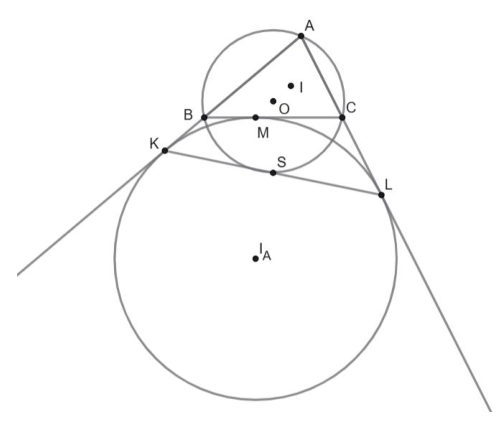
\includegraphics[width=0.5\textwidth]{mmo2526_P9.PNG} % 檔名不需副檔名，width設定寬度
    \end{figure}
    由旁切圓的性質可知
    $$
        AK=AL=\text{$\triangle{ABC}$的半周長}
    $$
    所以$\triangle{AKL}$是等腰三角形。因為$AI$是$\angle{KAL}=\angle{BAC}$的角平分線，$S$是$KL$的中點，所以$A$、$I$、$S$三點共線。
    由旁心的性質可知$A$、$I$、$I_A$三點共線，所以$A$、$I$、$S$、$I_A$四點共線。

    因為$S$是$AI$與$\triangle{ABC}$的外接圓交點，所以$S$平分含$S$點的弧$BC$，因此有$OS\perp BC$。

    因為$M$是旁切圓$\odot I_A$在$BC$上的切點，所以$I_AM\perp BC$。由此可知 $OS\parallel I_AM$。

    由雞爪定理知 $IS=I_AS=II_A/2$，結合$OS\parallel I_AM$，所以$I$、$M$、$O$三點共線可以等價於以下的命題一
    $$
        2R=2OS=I_AM=r_{A}
    $$
    其中$R$和$r_{A}$分別代表$\triangle{ABC}$的外接圓和$A$點所對的旁切圓半徑。

    由旁切圓半徑與外接圓半徑的三角函數關係
    $$
        r_A=4R\sin{\frac{A}{2}}\cos{\frac{B}{2}}\cos{\frac{C}{2}}
    $$
    可以把命題一等價於以下的命題二
    \begin{align*}
        &2\sin{\frac{A}{2}}\cos{\frac{B}{2}}\cos{\frac{C}{2}}=1\\
        \Leftrightarrow\quad& \sin{\frac{A}{2}}\left[\cos{\left(\frac{B+C}{2}\right)}+\cos{\left(\frac{B-C}{2}\right)}\right]=1\\
        \Leftrightarrow\quad& \sin{\frac{A}{2}}\left[\sin{\frac{A}{2}}+\cos{\left(\frac{B-C}{2}\right)}\right]=1\\
        \Leftrightarrow\quad& \sin{\frac{A}{2}}\cos{\left(\frac{B-C}{2}\right)}=1-\sin^2{\frac{A}{2}}\\
        \Leftrightarrow\quad& \sin{\frac{A}{2}}\cos{\left(\frac{B-C}{2}\right)}=\cos^2{\frac{A}{2}}
    \end{align*}

    另一方面，給合$IS=I_AS$和$S$為$KL$中點可知，所以$KILI_A$是平行四邊形。（對角線互相平分）
    
    又因為 $I_AK=I_AL$，所以$KILI_A$是菱形（鄰邊相等的平行四邊形），因此$I_K=I_AK=r_A$。

    作$\triangle{ABC}$的內切圓切$AB$與$D$點，易知 $DK=BC$，結合勾股定理可得
    \begin{align*}
        &r_A^2=IK^2=DK^2+r^2=BC^2+r^2\\
        \Leftrightarrow\quad& r_A^2-r^2=BC^2\\
        \Leftrightarrow\quad& \left(4R\sin{\frac{A}{2}}\right)^2\left(\cos^2{\frac{B}{2}}\cos^2{\frac{C}{2}}
        -\sin^2{\frac{B}{2}}\sin^2{\frac{C}{2}}\right)=\left(4R\sin{\frac{A}{2}}\right)^2\cos^2{\frac{A}{2}}\\
        \Leftrightarrow\quad& \cos{\left(\frac{B+C}{2}\right)}\cos{\left(\frac{B-C}{2}\right)}=\cos^2{\frac{A}{2}}\\
        \Leftrightarrow\quad& \sin{\frac{A}{2}}\cos{\left(\frac{B-C}{2}\right)}=\cos^2{\frac{A}{2}}
    \end{align*}
    因此命題二成立，原命題得證。
\end{mybox}
\end{document}